\documentclass{bioinfo}
\copyrightyear{2017} \pubyear{2017}
\usepackage{float}
\addtolength{\topmargin}{-.5in}
\addtolength{\textheight}{50pt}
\usepackage{multirow}

\access{Advance Access Publication Date: Day Month Year}
\appnotes{Application Note}

\begin{document}
\firstpage{1}

\title[short Title]{GPU accelerated KMC2}
\author[]{Huiren Li\,$^{\text{\sfb 1,}*}$, Anand Ramachandran\,$^{\text{\sfb 1}}$ and
Deming Chen\,$^{\text{\sfb 1,}*}$}
\address{$^{\text{\sf 1}}$Department of Electrical and Computer Engineering, University of
Illinois at Urbana-Champaign, Urbana, IL 61801, USA}

\corresp{}

\history{Received on XXXXX; revised on XXXXX; accepted on XXXXX}

\editor{Associate Editor: XXXXXXX}

\abstract{\textbf{Motivation:} K-mer counting is a popular pre-processing step in many
bioinforamtic algorithms. KMC2 is one of the most popular tools for k-mer counting. In
this work, we leverage the computation power of the GPU to accelerate KMC2. Our goal is to
reduce the overall runtime of many genome analysis tasks that use K-mer counting as an
essential step.\\
\textbf{Availability:} Source code is freely available at https://github.com/huiren/kmc2.\\
\textbf{Results:} We achieved 3.8x speedup using one GTX 1080 Ti with one CPU (Xeon
E5-2603)
thread and 5.2x speedup using one GPU with four CPU threads over a single CPU thread.\\
\textbf{Contact:} \href{dchen@illinois.edu}{dchen@illinois.edu}\\}

\maketitle

\section{Introduction}

K-mer counting refers to counting the frequencies of all k-length strings in a collection
of sequencing reads.
K-mer counting is a fundamental step for many bioinformatic algorithms, such as BLESS 2
\citep{Heo16} and Gerbil \citep{Mar17}.

The idea behind k-mer counting is very simple. A naive way to count k-mers would be similar 
to building a hash table of every k-mer mapped to the number of times that k-mer occurs 
in the given dataset. However, when the number of k-mers becomes very large, such as in 
the case of the human genome, this approach becomes impractical.

To make k-mer counting efficient and fast, different k-mer counting algorithms have been developed.
KMC2 \citep{Seb14} is a one of the most popular k-mer counting tools. KMC2 is designed to
be memory-efficient and fast while some other k-mer counting tools need tens of
gigabytes of memory like Jellyfish \citep{Mar11} and BFCounter \citep{Mel11}.

Even with tools like KMC2, k-mer counting would still take a substantial amount of time to
process. The original KMC2 was implemented purely using CPU.
In this work, we would like to exploit the computation power of GPU and further optimize
the running time of KMC2. We developed a memory-efficient GPU implementation of KMC2 for
acceleration.
We achieved a significant speedup over the original CPU implementation while maintaining a
small memory footprint.
%\enlargethispage{12pt}

\section{Approach}
There are two key concepts behind KMC2: signature and super k-mer.
A signature is lexicographically the smallest m-mer where m is smaller or equal to k.
Another constraint for a signature is that it cannot contain substring sequence AA and it
does not start with AAA or ACA.
A super k-mer is formed by consecutive k-mers which share the same signature.

KMC2 includes two major stages. In the first stage, super k-mers from the reads are 
distributed across bins stored on the disk, based on the signatures of the super k-mers. 
The use of super k-mers rather than k-mers allows reduction in disk footprint. This also 
helps reduce the memory footprint when each bin is opened in memory for further processing 
in the second stage. To ensure balanced distribution of super k-mers across the bins, 
during the first stage, KMC2 examines the signatures in the dataset to develop a balanced 
signature map as a preprocessnig step.

In the second stage, we process the bins one at a time. For each bin, we expand the super
k-mers stored in the bin. Then we sort the expanded k-mers, collect the k-mer counts in it 
and write the results to the output file.

In the following subsections, we will talk about our implementation in detail.
\begin{figure*}[t]
	\centering
	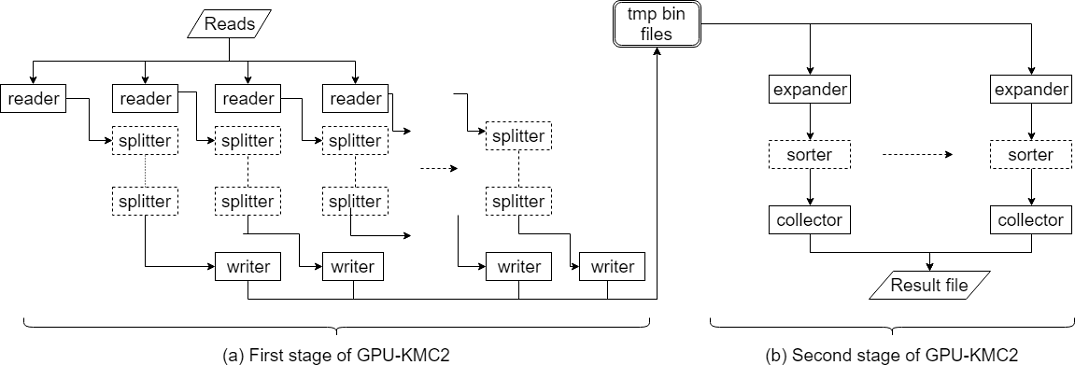
\includegraphics[scale=0.5]{kmc2.png}
	\caption{Overview of GPU acclerated KMC2. Rectangles with dotted lines are processes
	that are parallelized using CUDA.}\label{fig:01}
\end{figure*}
\enlargethispage{6pt}
\subsection{First Stage}
Figure~1\vphantom{\ref{fig:01}} (a) shows our implementation of the first stage.
In the first stage, the host will read the sequencing reads from the fastq file and store
it in a buffer.
When enough reads are stored in the buffer, it will pass the sequencing reads to the GPU
side for processing.
Each GPU thread is a splitter responsible for one sequencing read. The splitters
split the super k-mers from the reads and store them in a return buffer in gloabl memory on
the device.
After the return buffer is copied back to the host, it will be dumped into files 
representing the bins.

We have two options to implement the return buffer on the GPU side. We could
have a global buffer shared by all threads or each thread could have its own buffer.
Using the global buffer is more memory efficient but it requires a lock for every bin in
the buffer.
Although giving each thread its own buffer space avoids the pain of dealing with locks in
CUDA, it limits the number of reads we could process during each batch.
The later method turns out to be worse because of the large memory overhead it introduces.
Moreover, since we would process fewer reads during each batch of work, the GPU utilization
would be low.
\newpage

To minimize the running time of the first stage, we maximized the overlap between host and
device computation.
The readers and writers and writers (which couldn't be efficiently parallelized on the GPU)
 constitute the operations performed by the host.
As shown in Figure~1\vphantom{\ref{fig:01}}, when the kernels for splitters are running on
the device side, the host first writes the result of the previous batch to the disk (if
that batch exits) and then prepares the reads for the next batch.
Therefore, the idle time of the device is minimized.
Figure~1\vphantom{\ref{fig:01}} (a) shows the collaboration between GPU and CPU in
the first stage.
\subsection{Second Stage}
There are three main steps in the second stage.
The first one is expander; it is used to read the bins from the disk and pre-process the 
super k-mers. The second step is
a sorter to sort the result from the first step. The third step is a collector to collect
statistics from the sorted results and store it in the result file.
Figure~1\vphantom{\ref{fig:01}} (b) shows the implementation of the second stage.

The sorter uses radix sort which can be easily parallelized on GPU.
Therefore, a collaborative processing with both GPU and CPU is more efficient.
We used radix sort implemented in Thrust \citep{Jared} provided by NVIDIA to perform the 
sorting in the sorters on GPU.
Based on our analysis, the expander and collector may be parallelized efficiently across bins.
Since the number of bins is limited, they are good targets for parallelization using OpenMP on 
the host side. Using OpenMP parallelism for the expander and collector provides significant 
improvements in speedup of the second stage, in our observation.

According to our understanding, the parallelism in the second stage is mainly across the bins.
We used OpenMP to process multiple bins at the same time to exploit this level of parallelism.


\section{Results and Conclusion}
In order to evaluate the performance of the GPU acceleration for KMC2, we tested our
implementation against the original KMC2 \citep{Seb14}.

All experiments are done using Xeon E5-2603 v2 CPU and GeForce GTX 1080 Ti.
The testing is done using mouse genome with 40x coverage and read length equals to 100.
The results are summarized in Table~\ref{Tab:01} and Table~\ref{Tab:02}.

Compared to the original KMC2 implementation \citep{Seb14} running on a single CPU thread, 
our implementation that uses one GPU achieved an overall speedup of 4.03x when using a single 
CPU thread and 5.88x when using four CPU threads for k=40. Compared to the original KMC2 
implementation \citep{Seb14} running on 4 CPU threads, our implementation using a single GPU and 4 
CPU threads achieves a speedup of 1.37x and 2x in the best case (k=40). These accelerations are, 
respectively, 3.48x and 4.6x for k = 50.

We also compared our implementation of KMC2 to two other popular k-mer counting tools, JellyFish2 
and DSK for k=40. When the JellyFish2 and DSK implementations use 1 CPU thread, our implementation 
using 1 GPU and 1 CPU thread achieves 7.24x improvement over JellyFish2 and 5.85x over DSK. When we 
use 4 CPU threads, the numbers are, respectively, 4.32x and 3.03x. 

\begin{table}[H]
\processtable{K-mer counting results, baseline is KMC2 with one thread
\label{Tab:01}} 
{\begin{tabular}{|l|l|l|l|l|l|l|}
\hline
    \multirow{2}{*}{k-mer length=40} &
      \multicolumn{2}{c}{First Stage} &
      \multicolumn{2}{c}{Second Stage} &
      \multicolumn{2}{c|}{Total} \\
    & time & speedup & time & speedup & time & speedup \\
    \hline
    KMC2 (1 thread) & 127 & 1.0x & 307 & 1.0x & 435 & 1.0x  \\
    \hline
    KMC2 (4 threads) & 62 & 2.05x & 85 & 3.61x & 148 & 2.94x \\
    \hline
    GPU KMC2 (1 thread) & 23 & 5.52x & 85 & 3.61x & 108 & 4.03x \\
    \hline
    GPU KMC2 (4 threads) & 23 & 5.52x & 51 & 6.02x & 74 & 5.88x \\
    \hline
    DSK (1 thread) & N/A & N/A & N/A & N/A & 866 & 0.50x\\
    \hline
    DSK (4 threads) & N/A & N/A & N/A & N/A & 224 & 1.94x\\
    \hline
    JellyFish2 (1 thread) & N/A & N/A & N/A & N/A & 1072 & 0.41x\\
    \hline
    JellyFish2 (4 threads) & N/A & N/A & N/A & N/A & 320 & 1.36x\\
    \hline
\end{tabular}}{}
\processtable{K-mer counting results, baseline is KMC2 with one thread
\label{Tab:02}}
{\begin{tabular}{|l|l|l|l|l|l|l|}
\hline
    \multirow{2}{*}{k-mer length=50} &
      \multicolumn{2}{c}{First Stage} &
      \multicolumn{2}{c}{Second Stage} &
      \multicolumn{2}{c|}{Total} \\
    & time & speedup & time & speedup & time & speedup \\
    \hline
    KMC2 (1 thread) & 101 & 1.0x & 298 & 1.0x & 400 & 1.0x  \\
    \hline
    KMC2 (4 threads) & 42 & 2.40x & 80 & 3.73x & 123 & 3.25x \\
    \hline
    GPU KMC2 (1 thread) & 29 & 3.48x & 86 & 3.47x & 115 & 3.48x \\
    \hline
    GPU KMC2 (4 threads) & 29 & 3.48x & 58 & 5.16x & 87 & 4.60x \\
    \hline
\end{tabular}}{}
\end{table}

Note that the speedup in the first stage is the same disregard the number of CPU
threads we used because we are not using OpenMP in the first stage.
Moreover, the speedup we got using GPU with 4 CPU threads is not very significant.
The reason is that the sorters are not parallelized by OpenMP. Even multiple CPU threads
are running at the time, only one sorter kernel could be launched.
There is a large overhead in this process due to the serialized cudaMemcpy's and kernel
launched. Therefore, it prevented further performance gain.

\begin{thebibliography}{}

\bibitem[Deorowicz {\it et~al}., 2014]{Seb14}
Deorowicz,S.,Kokot,M.,Grabowski,S.,Debudaj-Grabysz,S. (2014). KMC 2: Fast and resource-
frugal k-mer counting, {\it Bioinformatics}, {\bf 00}, 1-21.

\bibitem[Heo {\it et~al}., 2016]{Heo16}
Heo,Y., Ramachandran,A., Hwu,W., Ma,J., Chen,D. (2016). BLESS 2: accurate, memory-
efficient and fast error correction method, {\it Bioinformatics}, {\bf 146}.

\bibitem[Jared {\it et~al}., 2015]{Jared}
Jared H., Nathan B. (2015). Thrust:https://thrust.github.io/

\bibitem[Marcais {\it et~al}., 2011]{Mar11}
Marcais,G., Kingsford,C. (2011).  A fast, lock-free approach for effi-
cient parallel counting of occurrences of k-mers, {\it Bioinformatics}, {\bf 146},
764-770.

\bibitem[Marius {\it et~al}., 2017]{Mar17}
Marius, E., Steffen, R., Matthias, M. (2017). Gerbil: a fast and memory-efficient k-mer
counter with GPU-support, {\it Algorithms for Molecular Biology}.

\bibitem[Melsted {\it et~al}., 2011]{Mel11}
Melsted,P., Pritchard,J.K. (2011). Efficient counting of k-mers in DNA sequences
using a bloom filter. {\it BMC Bioinformatics}, {\bf 12}, 333.

\bibitem[Rizk {\it et~al}., 2013]{Rizk13}
Rizk, G., Lavenier, D., Chikhi, R. (2013). DSK: k-mer counting with very low memory usage.
{\it BMC Bioinformatics}, {\bf 29}, 652-653.

\end{thebibliography}
\end{document}
